\documentclass[twoside,11pt,a4paper]{article}

% packages %%%%%%%%%%%%%%%%%%%%%%%%%%%%%%%%%%%%%%%%%%%%%%%%%%%%%%%%%%%%%%%%%%%%
\usepackage{graphicx,curves,float,rotating}

\usepackage{amsmath, amssymb, latexsym}  % math stuff
\usepackage{amsopn}                             % um mathe operatoren zu deklarieren
%\usepackage[ngerman]{babel}                     % otherwise use british or american
\usepackage[british]{babel}
\usepackage{theorem}                            % instead of \usepackage{amsthm}
\usepackage{dcolumn}
\usepackage{hyperref}
\usepackage{wrapfig}

% TODO remove before publishing
\usepackage{color}

% @ environment %%%%%%%%%%%%%%%%%%%%%%%%%%%%%%%%%%%%%%%%%%%%%%%%%%%%%%%%%%%%%%%%
\usepackage{xspace}                             % context sensitive space after macros
\makeatletter 
\DeclareRobustCommand\onedot{\futurelet\@let@token\@onedot}
\def\@onedot{\ifx\@let@token.\else.\null\fi\xspace}
\def\eg{{e.g}\onedot} \def\Eg{{E.g}\onedot}
\def\ie{{i.e}\onedot} \def\Ie{{I.e}\onedot}
\def\cf{{c.f}\onedot} \def\Cf{{C.f}\onedot}
\def\etc{{etc}\onedot} \def\vs{{vs}\onedot} 
\def\wrt{w.r.t\onedot} \def\dof{d.o.f\onedot}
\def\etal{{et al}\onedot}
\def\zB{z.B\onedot} \def\ZB{Z.B\onedot}
\def\dh{d.h\onedot} \def\Dh{D.h\onedot}
% %%%%%%%%%%%%%%%%%%%%%%%%%%%%%%%%%%%%%%%%%%%%%%%%%%%%%%%%%%%%%%%%%%%%%%%%%%%%%%%

%%%%%%%%%%%%%%%%%%%%%%%%%%%%%%%%%%%%%%%%%%%%%%%%%%%%%%%%%%%%%%%%%%%%%%%%%%%%%%%
%
%
%	Macros fuer neue Umgebungen
%
%
%%%%%%%%%%%%%%%%%%%%%%%%%%%%%%%%%%%%%%%%%%%%%%%%%%%%%%%%%%%%%%%%%%%%%%%%%%%%%%%
\newcommand*{\Frac}[2]{\frac{\displaystyle #1}{\displaystyle #2}}
\newlength{\textwd}
\newlength{\oddsidemargintmp}
\newlength{\evensidemargintmp}
\newcommand*{\hspaceof}[2]{\settowidth{\textwd}{#1}\mbox{\hspace{#2\textwd}}}
\newlength{\textht}
\newcommand*{\vspaceof}[3]{\settoheight{\textht}{#1}\mbox{\raisebox{#2\textht}{#3}}}
\newcommand*{\PreserveBackslash}[1]{\let\temp=\\#1\let\\=\temp}

\newenvironment{deflist}[1][\quad]%
{  \begin{list}{}{%
      \renewcommand{\makelabel}[1]{\textbf{##1}\hfil}%
      \settowidth{\labelwidth}{\textbf{#1}}%
      \setlength{\leftmargin}{\labelwidth}
      \addtolength{\leftmargin}{\labelsep}}}
{  \end{list}}


\newenvironment{Quote}% Definition of Quote
{  \begin{list}{}{%
      \setlength{\rightmargin}{0pt}}
      \item[]\ignorespaces}
{\unskip\end{list}}


\theoremstyle{break}
\theorembodyfont{\itshape}	
\theoremheaderfont{\scshape}

\newtheorem{Cor}{Corollary}
\newtheorem{Def}{Definition}
%\newtheorem{Def}[Cor]{Definition}



\newcolumntype{.}{D{.}{.}{-1}}


\pagestyle{headings}
\textwidth 15cm
\textheight 23cm
\oddsidemargin 1cm
\evensidemargin 0cm
%\parindent 0mm



%%%%%%%%%%%%%%%%%%%%%%%%%%%%%%%%%%%%%%%%%%%%%%%%%%%%%%%%%%%%%%%%%%%%%%%%%%%%%%%
%
%
%       Jetzt geht's los
%
%
%%%%%%%%%%%%%%%%%%%%%%%%%%%%%%%%%%%%%%%%%%%%%%%%%%%%%%%%%%%%%%%%%%%%%%%%%%%%%%%
\begin{document}


%% Der Befehl \LARGE beschreibt die Font-Groesse. Fuer die Groesse des
%% Schriftsatzes gibt es mehrere Befehle. Diese sind in aufsteigender
%% Reihenfolge:
%%
%%	\tiny 		\normalsize	\huge
%%	\scriptsize   	\large		\Huge
%%	\footnotesize	\Large
%%	\small		\LARGE
%%
%%
%% Um den Font zu aendern, stehen folgende Befehle zur Verfuegung:
%%
%%	\textrm{}	roman font
%%	\textsf{}	sans  serif
%%	\texttt{}	typewriter
%%	\textbf{}	bold series
%%	\textit{}	italic		(kursiv)
%%	\textsc{}	SMALL CAPS
%%	\textnormal{}	typeset text in the normal font
%%
%%
%% Mit dem Kommando \\  gibt man EXPLIZIT(!) an, dass man eine Zeile
%% umbrechen will (wie gesagt, normalerweise macht LaTeX das selbst).
%% Optional kann man hier \\ einen Wert angeben wie z.B. \\[4ex]
%% Damit legt man fest, wieviel Zwischenraum bis zur naechsten
%% Zeile bestehen soll. Das 'ex' steht fuer die Groesse des Symbols x.
%% Hier kann man auch die Einheiten 'pt' fuer Punkte, cm, ... benutzen.
%%
%% Der \vfill Befehl fuegt soviel Leerraum ein, das der restliche Text
%% bis an den unteren Rand gedrueckt wird (die Leerzeile davor wird
%% benoetigt). Der \newpage Befehl erzeugt einen EXPLIZITEN(!) Seiten-
%% umbruch. Da wir eine Leerseite haben wolllen wird mit '\ ' ein
%% Space-Symbol auf die Seite eingefuegt, so dass wir wieder einen
%% \newpage Befehl einsetzen koennen.


%%%%%%%%%%%%%%%%%%%%%%%%%%%%%%%%%%%%%%%%%%%%%%%%%%%%%%%%%%%%%%%%%%%%%%%%%%%%%%%
%
%
%               Title
%
%
%%%%%%%%%%%%%%%%%%%%%%%%%%%%%%%%%%%%%%%%%%%%%%%%%%%%%%%%%%%%%%%%%%%%%%%%%%%%%%%
\pagestyle{empty}

\begin{center}

    Rheinisch-Westf\"alische Technische Hochschule Aachen \\
    Lehrstuhl f\"ur Informatik 6 \\
    Prof. Dr.-Ing. Hermann Ney\\[6ex]
    Character-based Embeddings of Words with Recurrent Nets (for Neural Language Modeling)\\[12ex]  % auch Seminar Titel und Datum aendern!!!
    SS 2016\\[6ex]
   
    \LARGE
    \textbf{Character-based Embeddings of Words with Recurrent Nets} \\[6ex]
    \textbf{Article} \\[6ex] % Changed this
    \textit{Simon Gr\"atzer} \\[6ex]
    \Large
    Matrikelnummer 311673 \\[6ex]
    16.06.2016

    \vfill
    \Large Betreuer: Kazuki Irie
	    
\end{center}

\newpage
\ 
\newpage

%%%%%%%%%%%%%%%%%%%%%%%%%%%%%%%%%%%%%%%%%%%%%%%%%%%%%%%%%%%%%%%%%%%%%%%%%%%%%%%
%
%
%               Inhaltsverzeichnis / Tabellenverzeichnis / Abbildungsverz.
%
%
%
%%%%%%%%%%%%%%%%%%%%%%%%%%%%%%%%%%%%%%%%%%%%%%%%%%%%%%%%%%%%%%%%%%%%%%%%%%%%%%%
\pagestyle{headings}
\tableofcontents
\listoftables
\listoffigures
\newpage
\pagestyle{empty}
\ 
\newpage
\pagestyle{headings}

%%%%%%%%%%%%%%%%%%%%%%%%%%%%%%%%%%%%%%%%%%%%%%%%%%%%%%%%%%%%%%%%%%%%%%%%%%%%%%%
%
%
%               Inhalt
%
%
%%%%%%%%%%%%%%%%%%%%%%%%%%%%%%%%%%%%%%%%%%%%%%%%%%%%%%%%%%%%%%%%%%%%%%%%%%%%%%%

\section{Introduction}
\label{sec:Introduction}

%\subsection{Word Embeddings}

When neural networks process image or audio-data they usually work with rich, high-dimensional datasets.
For image data these might be vectors of individual pixel-intensities or for audio data vectors of power spectral density coefficients.
Natural language processing systems traditionally treat words as atomic symbols which are
encoded as simple indexes. For example 'apple' might become index $Id123$ and 'orange' becomes index $Id124$. This way the
encoding of the word data is arbitrary and contains no meaningful information regarding the relationships between word-symbols anymore.
In contrast to the dense representation of audio and image data, this way of encoding leads to data sparsity. Which means there is more data
required to sufficiently train our statistical models.

\begin{figure}[H]
\begin{center}
  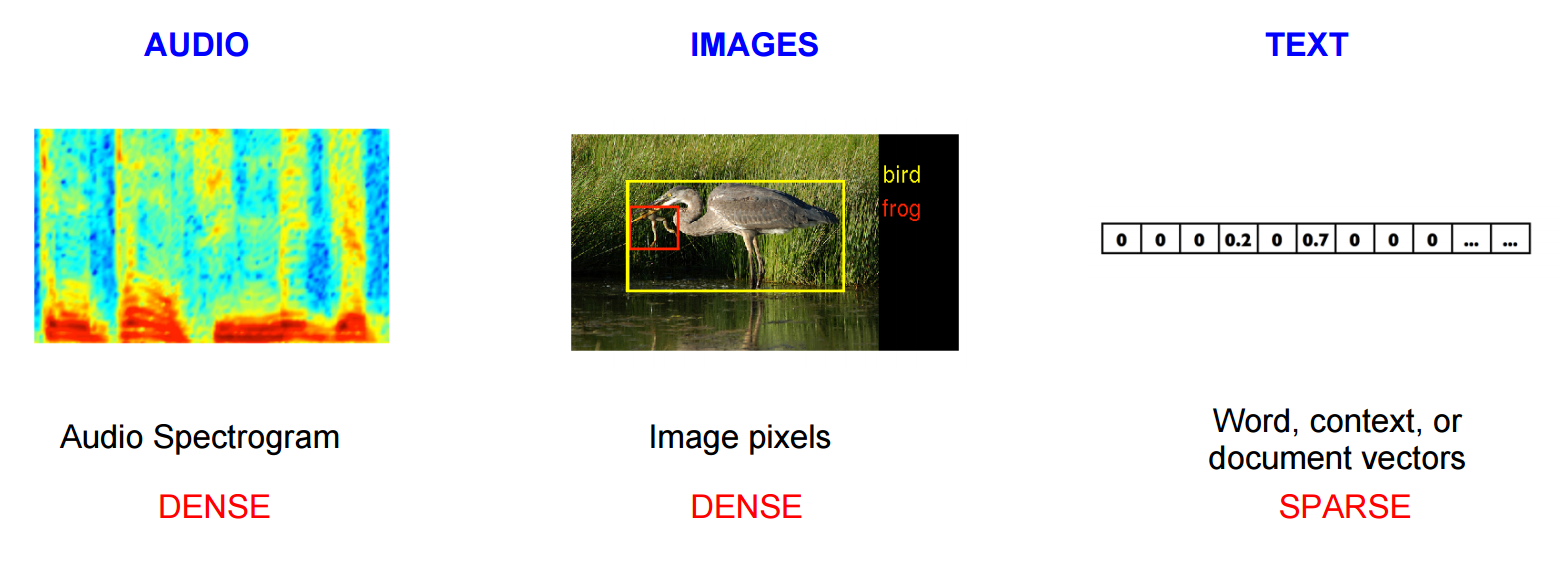
\includegraphics[width=\textwidth]{./img/audio-image-text}
  \caption{Comparison between the input datasets for different kinds of data (From~\cite{tensorflow:word2vec}).}
  \label{fig:audio-image-text}
\end{center}
\end{figure}

A statistical model can learn the relationships between word symbols (for example between 'apple' and 'apples') and leverage it for it's tasks.
Essentially we need to have a function which can take a word from the vocabulary and turn it into a feature vector.
The vectors are all in the same continuous vector space, in which we can now represent (embed) all words.
Ideally these feature vectors have a low dimension compared to the size of the vocabulary. Additionally words which have a
similar meaning (semantically similar) should be mapped to (geometrically) nearby points in the vector space.
They capture the intuitive understanding that words may be different 
or similar along a variety of dimensions in a quantifiable way.
An example can be seen in figure~\ref{fig:linear-relationships}, where some of these learned vectors representations
capture a semantic relationship between different words.

These vector representations of words are called "word embeddings" and a natural language processing 
system can use different methods to generate them.
All of these methods are based on the assumption that words which share semantic meaning tend to occur in the same contexts;
this is called the "Distributional Hypothesis"~\cite{Sahlgren2008}. 

\begin{figure}[H]
\begin{center}
  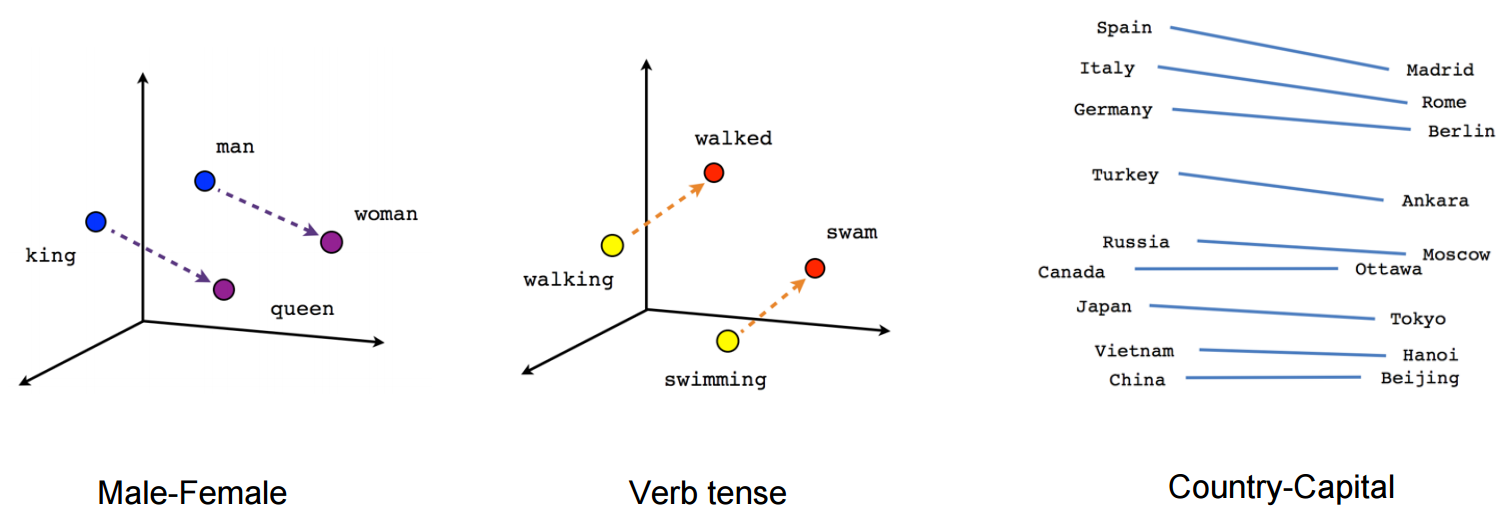
\includegraphics[width=\textwidth]{./img/linear-relationships}
  \caption{Visualization of word embeddings computed with the Skip-Gram model~\cite{DBLP:journals/corr/MikolovSCCD13}. 
  Vectors are projected onto 2 dimensions (Figure taken from~\cite{tensorflow:word2vec}).}
  \label{fig:linear-relationships}
\end{center}
\end{figure}

Formally we have our vocabulary $V$ and a function $f: V \rightarrow \mathbb{R}^d$ which maps $w \in V$ to a feature vector $\vec(w)$. 
A counting based approach to generate $f$ would be to perform a dimensionality reduction 
on a word co-occurrence matrix~\cite{DBLP:journals/corr/LebretL13}. The rows would then serve as the vectors.

However in this work we focus on recurrent neural networks to generate word embeddings. 
For example we will use the ability of neural nets to predict a word from the context (its neighbours) in which it appears. 
The first RNN will learn the vector embeddings as part of the larger processing system, 
in this case a natural network-based language model (NNLM).
By serving as the projection layer of the language model, the word embedding system is trained alongside with the rest of the model. 


% Many task's in Natural Language Processing (NLP) benefit from having a dense real-valued input vector, a good 
% embedding will improve outcomes for a lot of other tasks, like Part-of-Speech Tagging or language modeling.

% \subsection{Morphology}
% \label{subsec:Morphology}

% Short intro into morphology and why this is relevant to word embeddings.



% Text mit \"a, \"o, \"U, Stra{"s}e, Caf\'e.\\[4ex]


\section{Recurrent Neural Networks}

\subsection{Introduction}

Recurrent neural networks (RNN) are a class of neural networks where the connections in the graph can form directed cycles.
This is basically similar to existing neuronal structures like biological brains. 
The cyclic nature of the RNN-graph allows the net to "remember" previous inputs over amounts of time, 
as opposed to other classes of neural networks which are directed acyclic graphs (also called "feed forward")\\

This has the advantage that the RNN can act based on previous events, without having to receive all the context as input at the same time.
A simple example of an RNN can be seen in figure \ref{fig:RNN-rolled}, 
where the net processes the input value $x_t$ and outputs the value $h_t$.
The loop works essentially like copies of the same neural net chained up behind each other and passing it's current
output value $h_{t-1}$ to it's successor: $h_t = \sigma(W_{x} * x_t + W_{h} * h_{t-1})$ 
(Where $W_x$, $W_h$ are the parameters of the gate \textbf{A}).

Following this idea the RNN can be "unrolled" to show the processing of different inputs $x_i$ over time. An example of this can be seen in
the figure \ref{fig:RNN-unrolled}. This way an RNN looks just like a feed forward neural net. This way of looking at recurrent connections
will come up in the section~\ref{subsec:BPTT} where we discuss the training of RNN's.

\begin{wrapfigure}{r}{0.3\textwidth}
  \begin{center}
    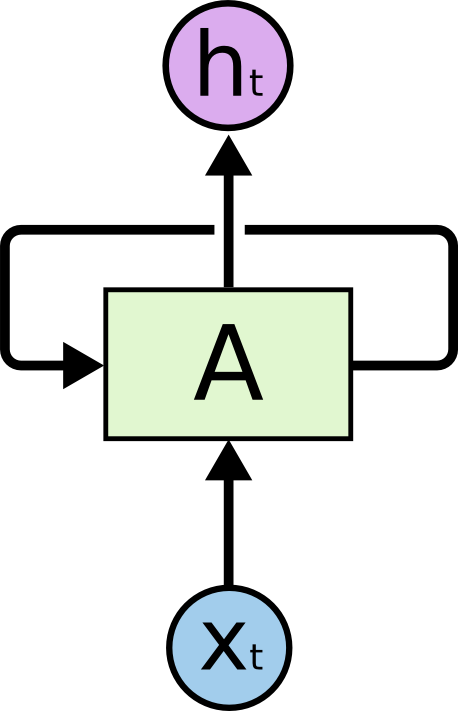
\includegraphics[width=0.4\textwidth]{./img/RNN-rolled}
  \end{center}
  \caption{A basic Recurrent Neural Networks, taking in the value $x_i$ and outputs the value $h_i$ (taken from~\cite{olah:lstm:2015})}
    \label{fig:RNN-rolled}
\end{wrapfigure}

\subsection{Training a RNN: Backpropagation Through Time}
\label{subsec:BPTT}

A common way to train neural networks is the so called "backpropagation of errors". It is a supervised learning method,
this requires having a known desired output value $y_t$ for every training input $x_t$. 
The measure of the difference between the desired and the 
actual output value of the net is the current error $E$, for example $E = \frac{1}{2} (h_t - y_t)^2$. 
The goal with backpropagation is to minimize the error $E$.

In other words we want to set every weight $w_{ij}$ of the neural net such that $E$ becomes minimal, 
the variable $w_{ij}$ denotes the weight for a connection between neurons i and j.
To minimize the error we can use the optimization method of "gradient descent". 
We calculate the gradient of $E$ with regards to the weights of the neural net: $\frac{\partial E}{\partial w_{ij}}$ and
then adjust every weight proportionally to the gradient:
\[
  \Delta w_{ij} = - \alpha \frac{\partial E}{\partial w_{ij}}
\]
In this formula $\alpha$ is a factor to control the speed of the learning process and prevent overfitting\\

We can't just apply backpropagation to an RNN, because this doesn't account for the recursive nature of some of the links. 
A simple solution to this is the method of Backpropagation Through Time (BPTT). As previously described, the recursive 
link in the RNN can be "unrolled" such that the network becomes a normal feed forward network, see figure \ref{fig:RNN-unrolled}. 
The RNN loop is unrolled $t$ times and now contains $t$ instances of $A$ with $t$ inputs. 
If we have some sample data each training pattern consists of
$\langle\mathbf{x}_0,\mathbf{y}_0,\mathbf{x}_{1},\mathbf{x}_{2},\dots,\mathbf{x}_{t},\mathbf{y}_{t}\rangle$, 
where ${y_0,\dots,y_t}$ are the desired outputs.
This sample can then be used for the training with backpropagation and gradient descend.

\begin{figure}[H]
\begin{center}
  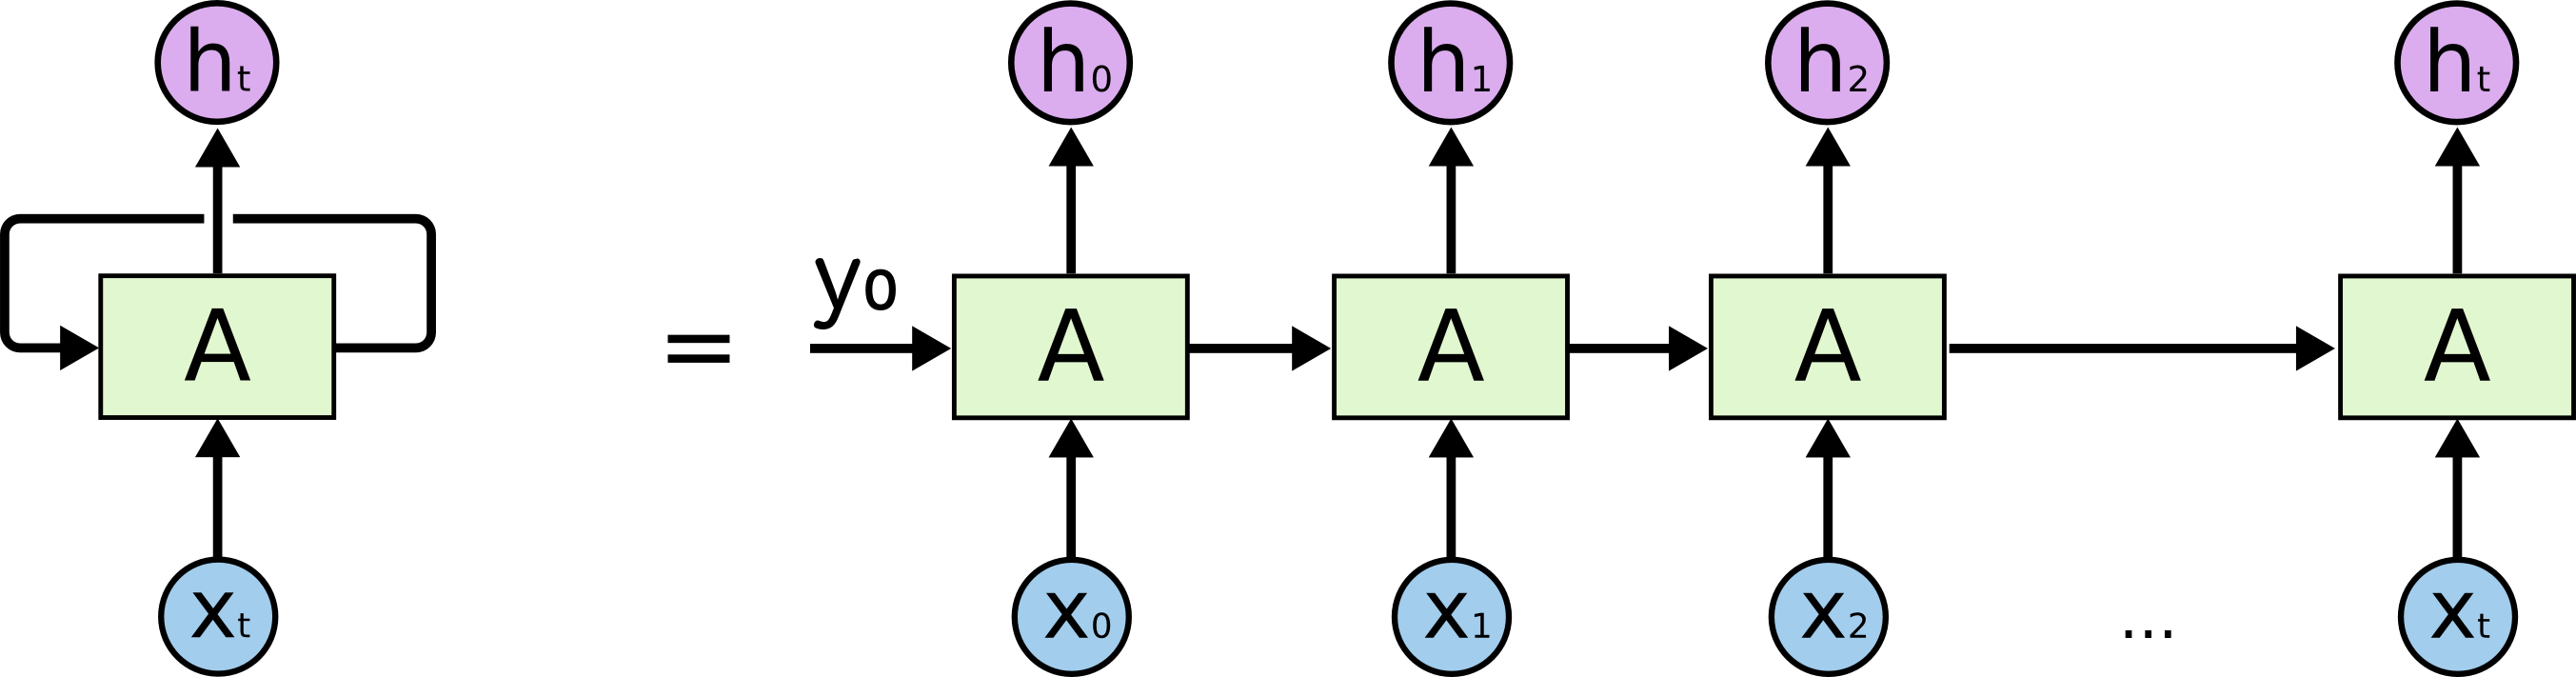
\includegraphics[width=\textwidth]{./img/RNN-unrolled}
  \caption{An unrolled recurrent neural network (taken from \cite{olah:lstm:2015}).}
  \label{fig:RNN-unrolled}
\end{center}
\end{figure}


\subsubsection{Vanishing gradient problem}

During training with backpropagation recurrent neural networks often suffer of the problem of vanishing gradients.
When using BPTT for training a RNN the error gets backpropagated through potentially a great number of layers. The magnitude
of the gradients of $E$ is affected by the weights and the derivatives of the activation function. If either of these amounts
to a factor of $< 1$ then the gradients can vanish over time, because we calculate the gradients with the
chain rule $(f\circ g)'=(f'\circ g)\cdot g'$.
This is a problem with a lot of common activation functions. For example the derivative 
of $\tanh(x)$ will be $< 1$ for all inputs $\neq 0$, 
the derivative of the sigmoid function is always $\frac{\partial sig(x)}{\partial x} \leq 0.25$. 
If a network has a lot of layers a lot of these small numbers get multiplied to calculate their gradient, and subsequently 
these layers train very slowly.
If the gradients can become larger than $1$ the gradients might become very big (exploding gradient problem).

There are a couple of solutions for this problem: With faster hardware the slow training of some layers may not be such a big issue anymore.
Another solution is to avoid recurrent connections with gradients $\neq 1$. This way there are not many factors where the
gradient can vanish. One such example is the LSTM network described in section~\ref{subsec:lstm}. 
The activation function in the recurrency of the LSTM is the identity function, with a derivative of $1$. Therefore the problems described 
above don't apply. There are other methods, but these are beyond our scope here.

%There are two factors that affect the magnitude of gradients - the weights and the activation functions (or more precisely, 
% their derivatives) that the gradient passes through.
%If either of these factors is smaller than 1, then the gradients may vanish in time; 
%if larger than 1, then exploding might happen. For example, the tanh derivative is <1 for all inputs except 0; 
% sigmoid is even worse and is always ≤0.25.


\subsection{Long-Short Term Memory}
\label{subsec:lstm}

A special form of RNN which is designed to "remember" inputs over arbitary distances and "forget" them when necessary.
They avoid the vanishing gradient problem are therefore very popular for tasks that involve any kind of classification,
processing or prediction of time-series data. This ability makes them very well suited for tasks like neural language modeling
or speech tagging where gap's between relevant inputs are likely.
A basic LSTM block will have 3 essential gates:

\begin{itemize}
\item Gate \(i_t\) to determine when to learn an input value
\item Gate \(f_t\) to determine if it should continue to remember or forget the currently stored value
\item Gate \(o_t\) to determine wether it should output the value.
\end{itemize}

The figure~\ref{fig:Long_Short_Term_Memory} below shows a simple LSTM gate, with arrows showing the flow of the values.
The gates with $\bigotimes$ calculate component-wise (Hadamard) product of their inputs. The activation function is usually 
the sigmoid function, except for the input/output gates marked with $\int$, which usually use the $\tanh$ function.

\begin{figure}[H]
\begin{center}
  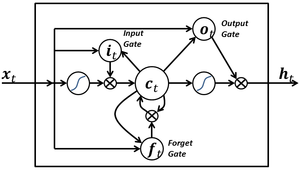
\includegraphics[width=0.7\textwidth]{./img/Long_Short_Term_Memory}
  \caption{A LSTM gate with input, output, and forget gate.}
  \label{fig:Long_Short_Term_Memory}
\end{center}
\end{figure}
Based on the input $x_t$, the remembered value $c_{t-1}$ and the output $h_{t-1}$ the input gates $i_t$, $f_t$ and $o_t$ can
decide how the LSTM behaves. If $i_t$ is close to zero, no input from $x_t$ is stored. If $f_t$ is close to zero,
the LSTM block will forget the stored value. Depending on $o_t$ the block outputs the stored value or not.
The output of $c_t$ is not directly fed through an activation function, so it doesn't automatically decay
over time.
Furthermore there are bias values $b_*$ added to all gates. Bias values can improve the performance of the LSTM compared to other RNN 
architectures according to~\cite{icml2015_jozefowicz15}.

Given the input vectors $x_1,\dots,x_m$ a LSTM computes the output sequence $h_1,\dots, h_{m+1}$ by iteratively applying the
following equations (The $W_*$ variables are the weight matrices of the gates):
\begin{equation}
\begin{aligned}  
  i_t &=\sigma(W_{ix} * x_t  + W_{ih} * h_{t-1} + W_{ic} * c_{t-1} + b_i) \\  
  f_t &=\sigma(W_{fx} * x_t  + W_{fh} * h_{t-1} + W_{fc} * c_{t-1} + b_f) \\
  o_t &=\sigma(W_{ox} * x_t  + W_{oh} * h_{t-1} + W_{oc} * c_t + b_o) \\  
  c_t &= f_t \odot c_{t-1} + i_t \odot \tanh(W_{cx} * x_t  + W_{ch} * h_{t-1} + b_c) \\ 
  h_t &= o_t \odot \tanh(c_t) 
\end{aligned}
\end{equation}

The sigmoid activation function is used for $i_t$, $f_t$, $o_t$ since it's $(0, 1)$ range is suited well for their particular gating decision: 
These gates 'decide' how much of the value to pass through, which is a 0\% to 100\% decision.
The $\tanh$ function is used as the output function, because it saturates at plus / minus one as opposed to zero and one for the sigmoid
function~\cite{Glorot10understandingthe}.

%As we will see, there are more complex variants of the LSTM. For example a possible addition is to feed the output value $h_{t-1}$
%into the gates $i_t$, $f_t$ and $o_t$. This way they can incorporate the actual output into their gating decision.
% It avoids the problem of vanishing gradients, because the gradient of the recurrency function will either be 0 or 1.

\subsection{Unsupervised training: Autoencoder}

An autoencoder transforms an input sequence into a code, and vice versa. 
An autoencoder consists of two parts: the encoder and the decoder. They can be defined as transitions $\phi$ and $\psi$, such that:\\
$\phi:\mathcal{X} \rightarrow \mathcal{F}$\\
$\psi:\mathcal{F} \rightarrow \mathcal{X}$\\
$\arg \min_{\phi,\psi} \|X-(\psi \circ \phi) X\|^2$\\
This will allow us to train a NN to generate word embeddings without the need for labeled data.
Given a sequence of words this NN can learn a mapping where the resulting feature vectors are similar for words which have a similar meaning. 

\begin{figure}[H]
\begin{center}
  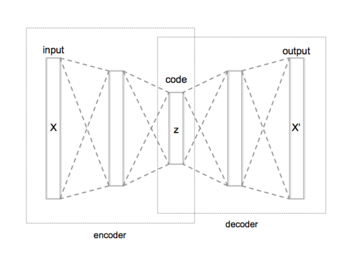
\includegraphics[width=0.5\textwidth]{./img/autoencoder_structure}
  \caption{An autoencoder NN with the encoding and decoding layer}
  \label{fig:autoencoder}
\end{center}
\end{figure}




\section{Introduction to Language Modeling}
\label{sec:language-modeling}

Language modelling is has the goal of determining a probability distribution on sequences of words (like sentences).
A (statistical) language model estimates a function which calculates the probability $p$ for the word sequence $w_1,\dots,w_m$:
\[
    p(w_1,\dots,w_m) = \prod_{i=1}^{m} p(w_i | w_1,\dots,w_{i-1})
\]
The fundamental challenge here is the dimensionality and vocabulary size of the data. For example to model the joint distribution
of 10 word sequences with a vocabulary $V$ size of 100.000 there are potentially $100000^{10} - 1$ 
free parameters~\cite{Bengio:2003:NPL:944919.944966}. 

% ==========================================================================================
\subsection{N-Gram Models}
\label{subsec:n-gram}

An n-gram is a contiguous sequence of n items / words from a given sequence of text or speech. Compared to the language model above,
we only try to estimate a probability distribution for the last $n$ words out of the sequence, we approximate the actual language model:
\[
p(w_1,\dots,w_m) = \prod_{i=1}^{m} p(w_i | w_1,\dots,w_{i-1}) \approx \prod_{i=1}^{m} p(w_i | w_{i-(n-1)},\dots,w_{i-1})
\]

So we assume we can approximate the probability for $w_i$ by replacing the context of the preceding $i - 1$ words with 
the context of the previous $n - 1$ words. Formally this is a $n - 1$ order Markov chain. % TODO citation, is it n or n-1 order?

For a 1-gram sequence this is called an unigram, a 2-gram s a bigram, n = 3 is a trigram and so forth.
One could estimate the conditional probabilities by counting all occurrences in the sample data:
\[
p(w_i\mid w_{i-(n-1)},\ldots,w_{i-1}) = \frac{\mathrm{count}(w_{i-(n-1)},\ldots,w_{i-1},w_i)}{\mathrm{count}(w_{i-(n-1)},\ldots,w_{i-1})}
\]
Of course this is very impractical, the number of possible sentences is too big. Additionally a training sample probably 
won't contain all possible combinations and therefore it's not possible to calculate estimations for all of them in this way.
In the next section we are going into some techniques used to mitigate this.

\subsubsection{Smoothing Techniques}

We need to be able to estimate word combinations wich we have previously not seen and assign a non-zero probability to them.
Some form of smoothing is necessary, the simplest possible solution is to just "add-one" to every word count.
This is called "Laplacian smoothing" and allows us to assume a count of 1 for unseen n-gram's. 

A better way is to use less context in these situations and to "Backoff". For example use a trigram instead of a 4-gram or a bigram and so on.
Additionally it can be a good solutions to mix results from unigram, bigram, trigram etc and linearly interpolate between them.
A more sophisticated way is to use neural networks, which represent words in a distributed way as 
a non-linear combinations of weights in a graph \cite{Hinton:1986:DR:104279.104287}.


% ==========================================================================================
\subsection{Perplexity}
\label{subsec:perplexity}

As we have previously seen, language modeling amounts to learning a posteriori probability distribution. 
Perplexity is a measure of how well a probability distribution predicts sample data. It can be 
interpreted as the number of choices per word position.
We can use it to formally judge how well a language model can predict the distribution. The exponent in the Perplexity term below
is the Entropy, it expresses the number of bits required to represent an event (in our case a word or character).

Formally Perplexity is defined as the sum of the inverse log-probabilities
\[
    2^{H(p)}=2^{-\sum_x p(x)\log_2 p(x)}
\]
Where $H(p)$ is the entropy~\cite{Shannon:1948} of the probability 
distribution $X$ of values ${x_1,\dots,x_n}$ with the probability mass function $p: X \rightarrow [0,1]$.

To minimize the perplexity value means to have a better fitting language model.

\subsubsection{Entropy}

Shannon~\cite{Shannon:1948} or Bit-Entropy is defined as $log_2(n)$ where $n$ is the number of possible outcomes. 
This assumes that all possible outcomes have the same probability. For a probability distribution 
we need to consider all three possible values ${x_1,\dots,x_n}$ it's likelihood of appearance and the entropy every possible outcome has.

The entropy of a value $x_i$ is dependent on it's self-information, which is inversely proportional to it's probability:
$I(x_i) = log(\frac{1}{p(x_i)}) = -log(p(x_i))$.
The self information of an intersection of two independent events $A$, $B$ is the sum of both: $I(A \cap B) = I(A) + I(B)$.
This is why the $log$ function is used to wrap $\frac{1}{p(x_i)}$.
In total the entropy for $X$ is defined as the expected information content of $X$: 
\[
    H(p) = E(I(X)) = -\sum_{i=1}^{n} p(x_i)\log_2 p(x_i)
\]

% ==========================================================================================
%\subsection{Skip-N-Gram Models}
% Possible cut depending on how the rest turns out

% The trouble with n-gram style language models is that they only consider the previous $n-1$ words regardless whether they have any real
% impact on the next word or not. The idea with the skip-n-gram model is to allow for a flexible context, which does not have to be
% the directly preceding words.
% \cite{DBLP:journals/corr/abs-1301-3781}


% ==========================================================================================
\subsection{Continuous space language models}
\label{subsec:cslm}

Continuous space language models can base their predictions on continuous representations of words. The word embeddings, which we will
discuss further in section~\ref{sec:c2w}, are a way to represent words in a continuous vector space. 
Continuous space embeddings help to alleviate the curse of dimensionality in language modeling, which arises out of the larger 
training texts. By representing the words in neural networks in a distributed way, 
we no longer have such a big issue with previously unseen word variations.

As with the simple counting based model from~\ref{subsec:n-gram} the neural network continuous space language models train to
estimate a probability distribution for the word $w_i$ given the linguistic context.
\[
    p(w_i|\text{context}) \forall w_i \in V
\]
As with the n-gram models the context can be for example limited to a fixed number of previous words. In contrast to the
simple counting model, a neural network can learn the complex non-local relationships between the word types in sequences.

\subsubsection{Classical Neural Language Model}

The classical neural language model architecture performs two tasks: First it projects the input words into the continuous vector space,
secondly it computes the language model probability for the given context. These task can be performed by two 
hidden layers~\cite{Schwenk:2007:CSL:1230156.1230409}. 
First every input word $w_i$ is encoded into vectors $1_{w_i}$ where
the entry corresponding to the index of $w_i$ within the vocabulary $V$ is $1$ and all other entries are $0$. 
This is then multiplied with a projection matrix $P \in \mathbb{R}^{|V| \times d}$ where $d$ is the dimension of the embeddings.
The embedding is obtained from $P$ by multiplying with a selection vector $1_{w_i}$, 
which is 1 at the word index: $e_{w_i}^W = P * 1_{w_i}$. The matrix $P$ is basically a lookup 
table for the word embeddings. 
The projections of all words in the context of the previous $n-1$ words are concatenated and form 
the first hidden layer (called the projection layer) of the NNLM.

A NNLM will always compute the probability for \textit{all} words contained in the vocabulary $V$. 
This is performed in combination by the second hidden layer and the output layer. 
The hidden layer will compute $d_j = f(\sum_{l = i-n+1}^{i-1} e_{w_l} * m_{lj} + b_l) \forall j = 1 \dots H$, 
where $H$ is the number of hidden neurons, $m_{lj}$ are the weights between the projection layer and the second hidden layer,
$b_j$ is the activation bias of neuron $j$. This combines all the word embeddings $e_w$ into an $H$ dimensional representation.
In the output layer this has to be scaled up to the vocabulary size again, 
by computing $z_k = \sum_{j = 1}^{H} v_{kj} * d_j + b_k \forall k = 1 \dots |V|$, where $v_{kj}$ are the weights of the output layer.
Since we have to transform this into a valid probability, the output layer uses a softmax function 
(introduced in section~\ref{subsec:softmax}), which will finally convert all $z_k$ values into probabilities $p_k$.
 
\begin{figure}[H]
\begin{center}
  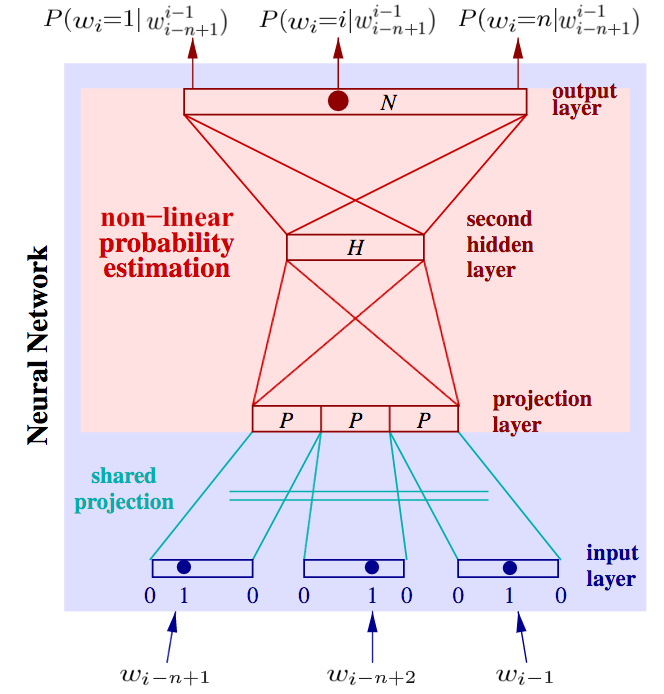
\includegraphics[width=0.7\textwidth]{./img/classic_nnlm}
  \caption{Architecture of a neural network language model, the context is denoted as $w_{i-n+1}^{i-1} = w_{i-(n-1)},\dots,w_{i-1}$.
  The output layer is a softmax over the vocabulary.
  (Figure taken from~\cite{Schwenk:2007:CSL:1230156.1230409}).}
  \label{fig:classic_nnlm}
\end{center}
\end{figure}

After training the resulting vector representations stored in $P$ can then be reused in other tasks.
This has the advantage that tasks with low amounts of training data can be trained together with tasks with larger amounts of data.
In section~\ref{subsec:language-model-c2w} we are going to discuss how to apply the word embeddings from section~\ref{sec:c2w} in
a neural natural language model, which is going to be structurally similar to the one presented here.

\subsubsection{Softmax Layer}
\label{subsec:softmax}

The Softmax function is a \textit{logistics function} and is often used as the final combining processing layer in neural
networks. It calculates a normalized exponential that 'squashes' the input such that the resulting vector entries add up to 1.
\[
    p_k = \sigma(\mathbf{z})_k = \frac{e^{z_k}}{\sum_{k=1}^{|V|} e^{z_k}}
\]
\begin{figure}[H]
\begin{center}
  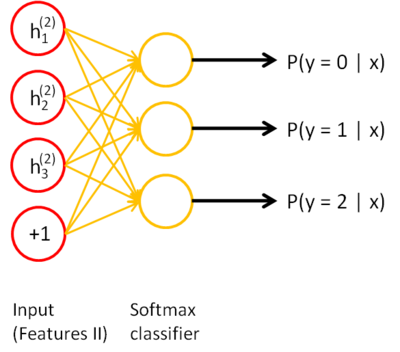
\includegraphics[width=0.5\textwidth]{./img/softmax_layer}
  \caption{Structure of a softmax layer in a neural network}
  \label{fig:softmax_layer}
\end{center}
\end{figure}

The property of the softmax layer is that the result of the outputs can be interpreted as posterior probabilities. 
This is useful in classification as it gives a valid posteriori propability measure for an n-gram model.
A softmax layer transforms the results of a hidden layer into a probability distribution for neural language models. The NNLM assigns the
probability given the context: $p_k = p(w_i = k | w_{i-n+1}^{i-1})$.

\subsubsection{Out of Vocabulary Token}

Since the softmax can only be computed for known words included in the vocabulary set $V$ it is not possible to handle words
not included in $V$ during testing.
These words are \textbf{Out Of Vocabulary} (OOV), the solution is to replace all of them with an special token word.
The probability for this OOV token can be learned during the training stage, by replacing word types with low frequencies with the $<$OOV$>$ token.
During test time we can now use the $<$OOV$>$ probabilities for any word not in the vocabulary $V$~\cite{DBLP:journals/corr/LingLMAADBT15}.

For a language modeling task where there is not a closed Vocabulary, we will almost certainly encounter words which are not known from
our training vocabulary set. It is therefore essential to apply a strategy like the above one to have a robust estimation
for OOV words.


\section{Character-based Word-Embeddings}
\label{sec:c2w}

\subsection{Introduction}

% Feeding character sequences to bidirectional LSTMs

The Compositional Characters to Word (C2W) Model is a new way to generate word embeddings 
presented by~\cite{DBLP:journals/corr/LingLMAADBT15}.
The input of the C2W model is a single word $w$, and we want to get a $d$-dimensional vector by which to represent $w$.
The basic idea is to let two LSTMs 'read' the word, by feeding them the word as a sequence of characters forwards and backwards.
The two resulting output states are then combined into the vector representation of the word.
%A commonly previously used approach is to treat the word embeddings as optimizable parameters
%in some kind of language model. 

The previous approach to build a NNLM as presented in~\ref{subsec:cslm} has some drawbacks which the C2W seeks to avoid:
\begin{enumerate}
  \item Each word embedding vector is independent. A word lookup table cannot generate representations for an unknown word, 
        even though it might have seen similar words before.
        A model might capture the linear correspondence of \textit{cat} and \textit{apple} compared to \textit{cats} and \textit{apples}, 
        but it doesn't capture that the added \textit{s} is responsible for this transformation. 
        It can't compute the same for a previously unseen plural word, even though it might know the singular version.
  \item For a large vocabulary it becomes impractical to actually store all word embeddings in a table.
\end{enumerate}
The C2W model avoids the first problem by breaking down words into their components. These components are then composed
back into the the representation of the word. There are previous efforts (\cite{Luong-etal:conll13:morpho}, \cite{DBLP:journals/corr/BothaB14}) 
which explore this idea, by breaking up words into their \textit{morphemes}. A morpheme is the smallest grammatical unit of a language 
e.g.\ "Unbreakable" comprises three morphemes: un-, -break-, and -able.
The downside of this approach is that you need a morphological analyzer to break down words. The C2W avoid this dependency by
breaking down words directly into characters.

\begin{wrapfigure}{r}{0.5\textwidth}
  \begin{center}
    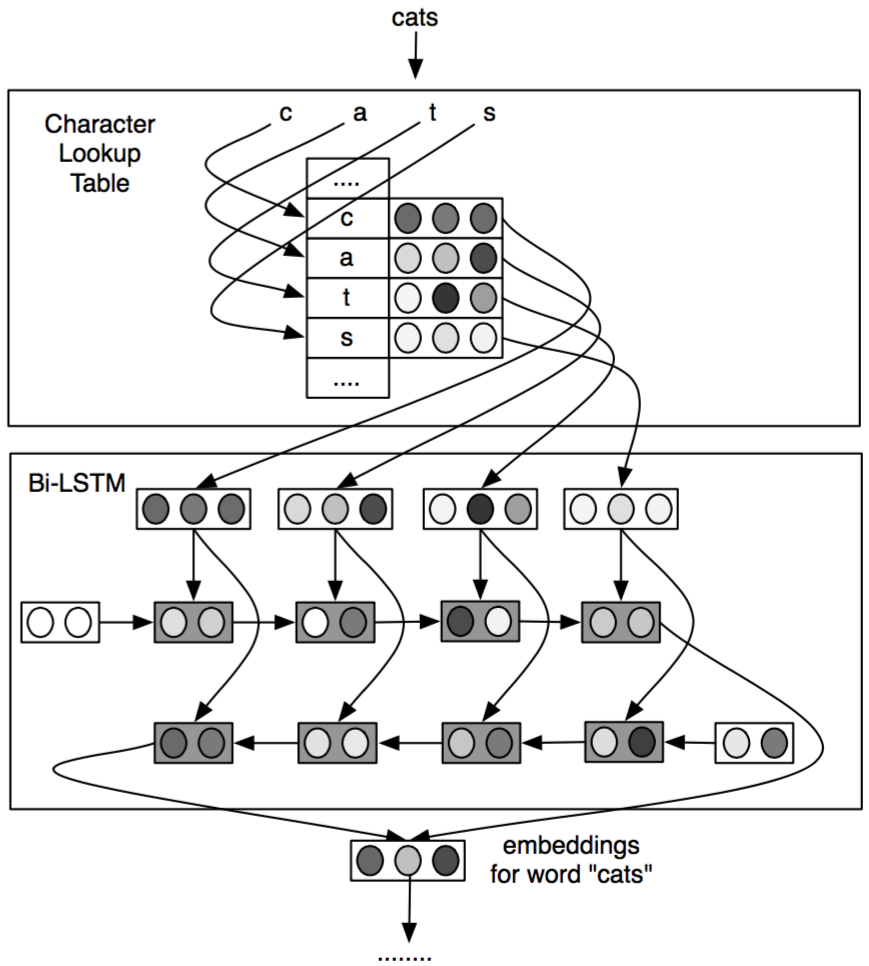
\includegraphics[width=0.5\textwidth]{./img/bi-lstm-emeddings}
  \end{center}
  \caption{Illustration of the lexical Composition Model (from~\cite{DBLP:journals/corr/LingLMAADBT15})}
\end{wrapfigure}

\subsection{Character Lookup Table}

The first processing steps involves a table of $d_C$ parameters for each character from a predefined character alphabet $C$.
Each word $w$ is decomposed into it's characters $c_1, \dots. c_m$.
Every input character gets transformed into a real-valued feature vector representation $e_{c_j}^C \in \mathbb{R}^{d_C}$.
The feacture vectors are stored in a projection layer $P_C \in \mathbb{R}^{d_C \times |C|}$ (Which is basically a lookup table for characters).
For each $c_j$ we can define the projection of our character as $e_{c_j}^C = P_C * 1_{c_j}$. In this equation the $1_{c_j} \in {0, 1}^{d_C}$ 
is a vector where all entries are zero except the entry corresponding to the index of the character$c_j$. 
The resulting sequence of character representations $e_{c_1}^C, \dots, e_{c_m}^C$ is then fed into the Bi-LSTM layer~\ref{subsec:bi-lstm}
in normal and reversed order.

\subsection{Bidirectional LSTM Layer}
\label{subsec:bi-lstm}

The second layer of the C2W model is a bidirectional LSTM layer~\cite{DBLP:journals/nn/GravesS05} as explained in section~\ref{subsec:bidir-rnn}. 
This consists of two LSTM blocks:
\begin{enumerate}
  \item The forward LSTM ($f$) which receives the sequence of character representations $e_{c_1}^C, \dots, e_{c_m}^C$
  \item The backward LSTM ($b$) which receives as input the reverse sequence $e_{c_m}^C, \dots, e_{c_1}^C$
\end{enumerate}
A LSTM has the parameter set $\mathcal{W} = \{W_{ix},\dots,W_{ch},b_i,\dots,b_o\}$,
there are two separate parameter sets for each LSTM block: One for the forward LSTM ($\mathcal{W}^f$) and one for the backward ($\mathcal{W}^b$) LSTM.
These basic equations are applied for every input character vector $e_{c_j}^C$, in the two LSTM blocks. 
Each LSTM replaces the parameters with the ones from $\mathcal{W}^f$ or $\mathcal{W}^b$ respectively.
\begin{equation}
\begin{aligned}  
  i_j &=\sigma(W_{ix} * e_{c_j}^C  + W_{ih} * s_{t-1} + W_{ic} * c_{j-1} + b_i) \\  
  f_j &=\sigma(W_{fx} * x_j  + W_{fh} * s_{j-1} + W_{fc} * c_{j-1} + b_f) \\
  o_j &=\sigma(W_{ox} * x_j  + W_{oh} * s_{j-1} + W_{oc} * c_j + b_o) \\  
  c_j &= f_j \odot c_{t-1} + i_j \odot \tanh(W_{cx} * x_j  + W_{ch} * s_{j-1} + b_c) \\ 
  s_j &= o_j \odot \tanh(c_j) 
\end{aligned}
\end{equation}
The forward LSTM yields the forward state sequence $s_{1}^f, \dots, s_{m}^f$ and the backward LSTM yields the state sequence $s_{m}^b, \dots, s_{1}^b$.

\subsubsection{Bidirectional LSTM's}
\label{subsec:bidir-rnn}

The idea of a bidirectional recurrent neural network (BRNN) is to present every input sequence forwards and backwards to two separate
recurrent neural networks~\cite{IEEE:journals/singals/Schuster1997}.
Both networks are connected to the same output layer. This way the complete network has access to sequential information 
about all inputs before and after the current one.
This is illustrated in figure~\ref{fig:brnn-unfolded}, where the complete input is provided to the RNN twice (forwards and backwards).
\begin{figure}[H]
\begin{center}
  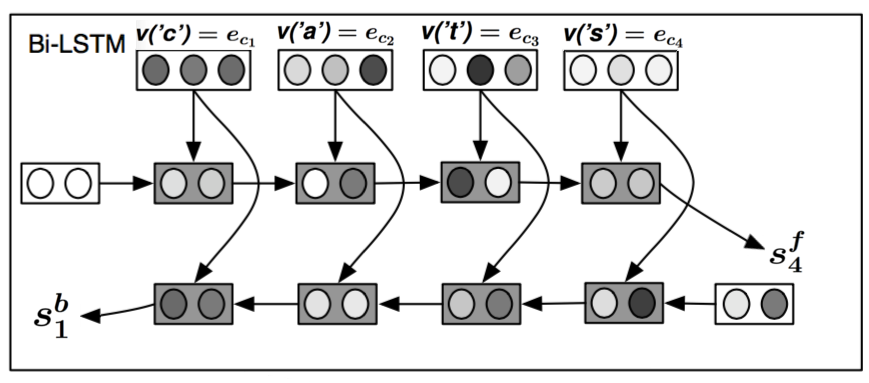
\includegraphics[width=\textwidth]{./img/brnn-unfolded}
  \caption{A generic BRNN unfolded for three timesteps (From~\cite{IEEE:journals/singals/Schuster1997}).}
  \label{fig:brnn-unfolded}
\end{center}
\end{figure}

The advantage of a BRNN is that there is no need to anymore manually specify how much context is 
used anymore (for example by having fixed-sized overlapping time-windows).
The net can decide to use as much or as little of the context as required. 
This can improve the results in sequence learning tasks, where the context can be previded in a "semi-online" fashion.
For example in online speech recognition an output after every sentences is fine~\cite{DBLP:journals/nn/GravesS05}. 

% Given the input vectors x1,...,xm, a LSTM computes the state sequence h1, . . . , hm+1 by it- eratively applying the following updates:



\subsection{Combining Forward-Backward Features}

Finally the last states of the forward sequence $s_{m}^f$ and the backwards sequence $s_{1}^b$
are linearly combined into the resulting word embedding $e_{w}^C$:
\[
  e_{w}^C = D^f s_{m}^f + D^b s_{0}^b + b_d
\]
The variables $D^f, D^b, b_d$ are the weights which determine how the states are combined.

Compared to using a lookup table computing $e_{w}^C$ is relatively expensive, but since the value only depends on
the word itself the value can be cached. This can be used for frequently occuring words to reduce the computational load.
At the same time not all words have to be cached, which reduces the amount of storage required for a large vocabulary.
\section{Applying the C2W model}

\subsection{Language Modeling}
\label{subsec:language-model-c2w}

In this section we use the C2W model and a recurrent LSTM to perform language modeling as 
described in~\cite{DBLP:journals/corr/LingLMAADBT15}.
The neural network is going to compute the log propability $\log[ p(\mathcal{w}) ]$ of the 
sentence $\mathcal{w} = (w_1, \dots, w_m)$. As previously discussed in section~\ref{sec:language-modeling} this can be 
decomposed into the sum of the conditional log probabilities $log[ p(w_1,\dots,w_m) ] = \sum_{i=1}^{m} log[ p(w_i | w_1,\dots,w_{i-1}) ]$.
This model will compose the previously described word representations of $w_1,\dots,w_{i-1}$ to compute 
$log[ p(w_i | w_1,\dots,w_{i-1}) ]$ using a LSTM unit.
The model is shown in figure~\ref{fig:c2w-language-model}. The first stage can use either the embeddings generated with the C2W model
$f(w_i) = e_{w_i}^C $ or simply word lookup tables $e_{w_i}^W = P * 1_{w_i}$.

Every time we input a new word $w_i$ from the sequence we get the LSTM state $s_i$. The state $s_i$ is then used to predict word $w_{i+1}$.
The state $s_i$ is projected into a vector of size $|V|$ (the vocabulary size). The softmax is a $d \times V$ table, 
which encodes the likelihood of every word type in the vocabulary in a given context. 
The softmax layer will ensure a valid log probability distribution. This way we can choose the word type with the maximal likelihood.
Maximizing the conditional log-likelihoods during training will improve the modeling 
of $p(\mathcal{w})$~\cite{DBLP:conf/interspeech/MikolovKBCK10}.
More details regarding the softmax layer are explained in section~\ref{subsec:softmax}.

\begin{figure}[H]
\begin{center}
  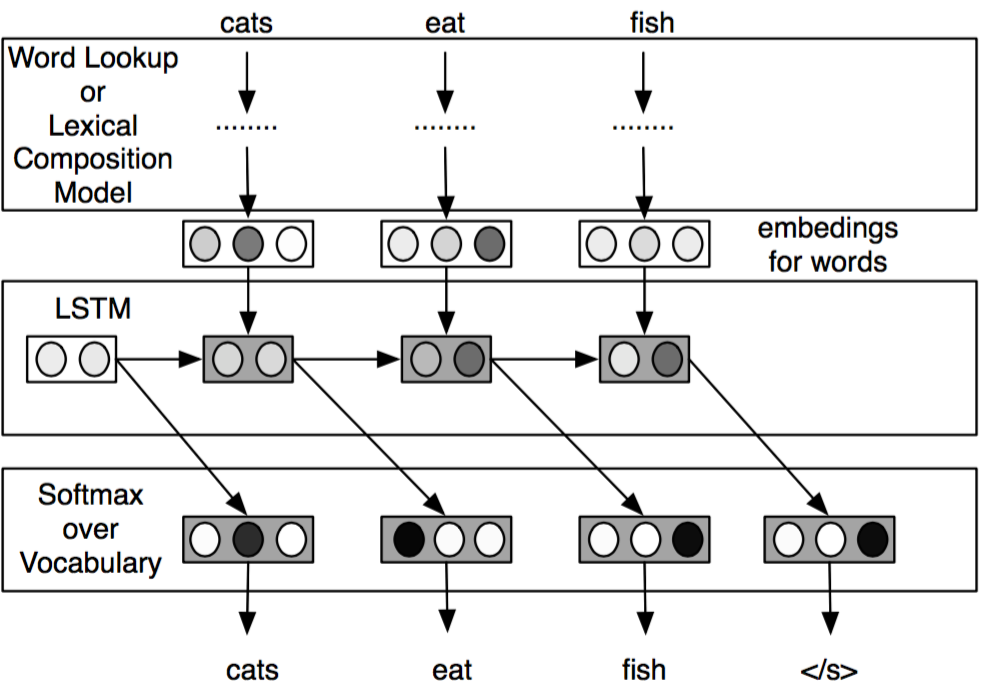
\includegraphics[width=0.6\textwidth]{./img/c2w-language-model}
  \caption{Neural network for language model. The C2W model is at the top, the word embeddings are then fed into an recurrent LSTM.}
  \label{fig:c2w-language-model}
\end{center}
\end{figure}


\subsubsection{Evaluation}

The original paper~\cite{DBLP:journals/corr/LingLMAADBT15} compares the performance of the language model 
in terms of it's perplexity~\ref{subsec:perplexity}. To minimize the perplexity value means to have a better fitting language model.
Perplexity cannot be used to compare models with different vocabularies,
since there are fewer outcomes in the softmax, the global perplexity can decrease.

In table~\ref{tab:perplexity} the perplexities and the parameter counts are displayed for different language models.
The language model performance is tested on English, Portuguese, Catalan, German and Turkish; the data is extracted from wikipedia.
Every word embedding $e_{w} \in \mathbb{R}^{d_w}$ is going to have $d_w = 50$ parameters.
Therefore the model using a lookup table of word embedding contains at least $d_w \cross |V|$ parameters.
The parameter count for the language model using C2W based embeddings depends on a few things. The number of parameters for each character
representation $d_C = 50$, and the number of parameters $d_{CS} = 150$ in the LSTM state $s_i$. The C2W model contains 8 matrices of 
size $d_{CS} \cross d_C + 2d_{CS}$ (One for each of the 4 decision gates in both LSTM's). Additionally there is the character lookup table 
which has an entry for every character in the language $d_C \cross |C|$. For English and 618 this works out to $15000 + 30900$ parameters.

\begin{table}
\begin{center}
\begin{tabular}{ l l l l l }
  \hline
             & \multicolumn{3}{|c|}{Fusional} &   \multicolumn{3}{|c|}{Agglutinative} \\ \hline
  Perplexity   & English & Portugese & Catalan & German & Turkish \\
  %5-gram KN    & 70.72   & 58.73     &   39.83 & 59.07  & 52.87   \\
  Word Lookup  & 59.38   & 46.17     &   35.34 & 43.02  & 44.01   \\
  C2W Model    & 57.39   & 40.92     &   34.92 & 41.94  & 32.88   \\
  #Parameters  &         &           &         &        &         \\
  Word Lookup  & 4.3M    & 4.2M      &  4.3M   & 6.3M   & 5.7M   \\
  C2W Model    & 180K    & 178K      &  182K   & 183K   & 174K   \\

\end{tabular}
\end{center}
\caption{Perplexities of different language models and the test configuration (From~\cite{DBLP:journals/corr/LingLMAADBT15}).}
\label{tab:perplexity}
\end{table}

% ==========================================================================================
\subsection{Part-of-Speech Tagging}

Part-of-Speech tagging is the process of labeling words as corresponding to a particular part of speech. A simple tagging would be
to identify words as nouns, verbs, adjectives, adverbs, etc.
The model receives a number of words $w_1,\dots,w_m$ as input, and transforms them into word embeddings. These embeddings are then processed
in a bidirectional LSTM layer, just as described in section~\ref{subsec:bidir-rnn}. 
In contrast to the combining layer of the C2W model, we don't just use the final state of the LSTM output states, but all states.
The forward states $s^f_0,\dots,s^f_m$ and the backward states  $s^n_m,\dots,s^b_0$ are combined with  $l_i = \tanh(L^f s_i^f + L^b s^b_i + b_l)$.
Where $L^f$, $L^b$, $b_l$ are the parameters of the combining layer. The output label for each word $w_i$ is then obtained from a softmax layer over
all word labels.

\begin{figure}[H]
\begin{center}
  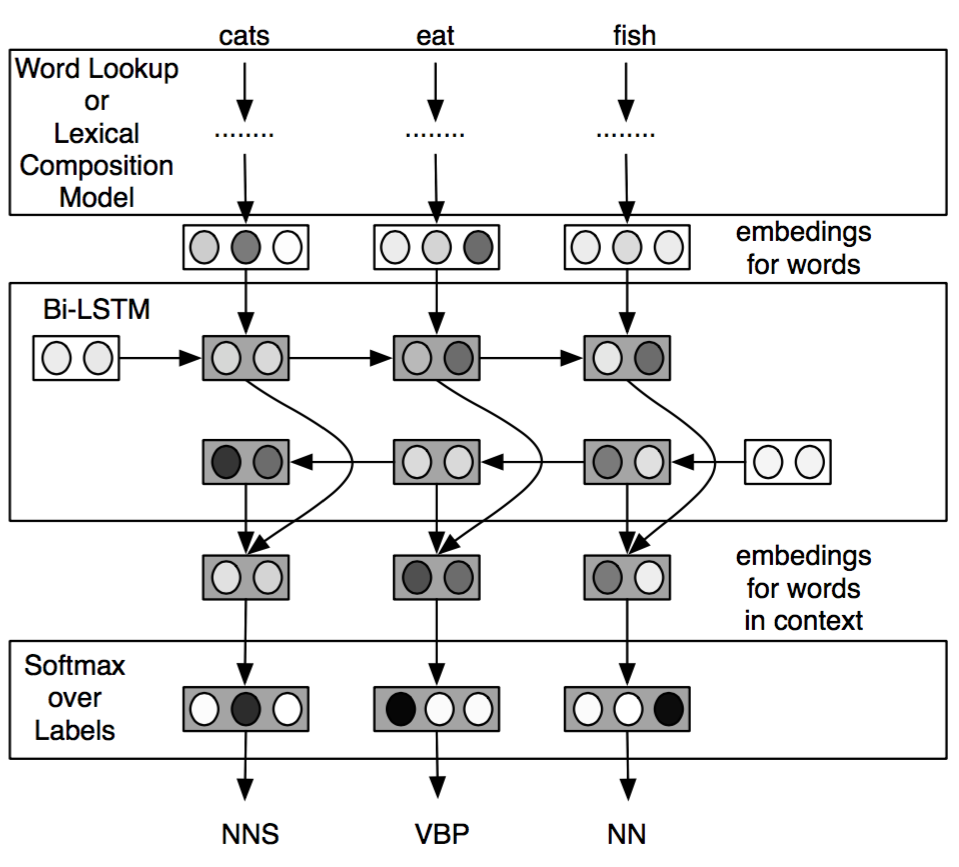
\includegraphics[width=0.6\textwidth]{./img/part-of-speech}
  \caption{The arhitecture of the NN for part-of-speech tagging (From~\cite{DBLP:journals/corr/LingLMAADBT15}).}
  \label{fig:c2w-language-model}
\end{center}
\end{figure}

\subsubsection{Evaluation}

The POS tagging is evaluated on the same languages as before. We compare the POS model with word embeddings from a lookup table
as well as Stanford’s POS tagger with the C2W based POS tagger.
\begin{table}
\begin{center}
\begin{tabular}{ l l l l l }
  \hline
  System       & \multicolumn{3}{|c|}{Fusional} &   \multicolumn{3}{|c|}{Agglutinative} \\ \hline
               & English & Portugese & Catalan & German & Turkish \\
  %5-gram KN    & 70.72   & 58.73     &   39.83 & 59.07  & 52.87   \\
  Word Lookup  & 96.97   & 95.67     &  98.09  & 97.51  & 83.43   \\
  C2W Model    & 97.36   & 97.47     &  98.92  & 98.08  & 91.59   \\
  Stanford     & 97.32   & 97.54     &  98.76  & 97.92  & 87.31  \\

\end{tabular}
\end{center}
\caption{Accuracy of the POS tagging in percent (From~\cite{DBLP:journals/corr/LingLMAADBT15}).}
\label{tab:pos-eval}
\end{table}


% ==========================================================================================
\subsection{Morphological inflection generation} 

Another application of C2W like model beyond language modeling is the morphological inflection generation~\cite{DBLP:journals/corr/FaruquiTND15}.
The goal is to perform a lingustic transformation some examples of the inflections which this model seeks to 
generate can be seen in table~\ref{tab:inflections}. First stage is the \textbf{encoder}:\\
This part of the model is eqvivalent to the C2W model: Each word $w$ is broken up into it's characters $e_{c_1}^C, \dots, e_{c_m}^C$.
Then a bidirectional LSTM layer is used and th result is composed into $e_{w}$.
Second part is the \textbf{decoder}:\\
This is a LSTM unit which will sequentially receive the word characters as input combined with the previous output and the word vector.
Every output state is computed as $s_t = g(s_{t-1}, \{e_{w}, y_{t-1}, x_t\})$. Where $g$ is the decoder LSTM unit,
$s_t$ is the LSTM output, $y_{t-1}$ the actual character output and $x_t$ is the current input character.
Since the input word might be shorter than the output, onece the input sequence runs out of characters we feed in an $\epsilon$ character
indicating null input: $x_t = \epsilon$. The vector representation for the $\epsilon$ character is learned just like in the C2W model.


\begin{figure}[H]
\begin{center}
  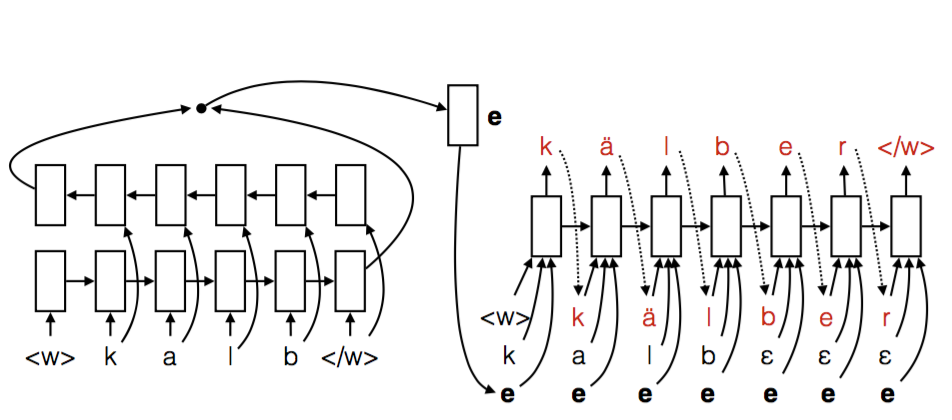
\includegraphics[width=\textwidth]{./img/inflection-generatior}
  \caption{A endoder decoder structure for inflection generation}
  \label{fig:inflection-generatior}
\end{center}
\end{figure}

\begin{table}
\begin{center}
\begin{tabular}{ l l l l }
  \hline
             & singular & plural \\ \hline
  nominative & Kalb & K\"alber \\
  accusative & Kalb & K\"alber \\
  dative & Kalb & K\"albern \\
  genitive & Kalbes & K\"alber \\
\end{tabular}
\end{center}
\caption{Example of an inflection table for the word Kalb (calf, German).}
\label{tab:inflections}
\end{table}

Converting the word embeddings from a C2W like model back into inflected versions of the word 
as discussed in Faruqui et al. \cite{DBLP:journals/corr/FaruquiTND15}

% Comparison of current LSTMs based word embeddings with the character based method from Santos et al. \cite{DBLP:conf/icml/2014}

% Dies ist ein laufender-Text mit Einsteins Formel $E = m \cdot c^2 $.

% Eine etwas kompliziertere Formel:
%\[
%     a \Frac{1 - q^{n+1}} {1-q}  =  \sum_{i=0}^{n} aq^{n} \qquad
%     \text{mit\ } \quad a,q \in \mathcal{R},  q \neq 1
% \]

%% Mit dem Befehl \mathcal erzeugt man ein kaligraphisches R im
%% mathematischen Modus. Der Befehl \neq erzeugt ein Ungleichheits-
%% Will man Formeln durchnumerieren, so kann man die equation-array
%% Umgebung benutzen.
%%

\section{Conclusion}

The concept of generating word embeddings by composing characters shows that it is possible to reach
state of the art results, with a magnitude less paramaters.
Manual engineering of features is not a necessity even for such tasks as Part-Of-Speech tagging.
As the experiments in~\cite{DBLP:journals/corr/LingLMAADBT15} show, lexical features can
can be learned automatically by the language model. Vocabulary-sized word lookup-tables
can be reduced to one (much smaller) character lookup table which avoids redundancies.
This allows the model to scale better with
larger amounts of training data. This is an additional advantage over similar approaches using 
morphenes as the atomic unit of words.
Using characters as the atomic unit of choice makes the application of the C2W model simple for many languages.
The nature of the C2W model also allows the handling of nonce words, which is not possible with other approaches.
The increased computational cost when using the C2W model compared to lookup tables is shown to be
insegnificant in many applications. For example in lagnuage modeling the computations in the intitial projection 
layer are insignificant compared to the computations in the softmax layer.




%% Tabellen werden mit der tabular Umgebung erzeugt. Mit der table
%% Umgebung werden wir unserer Tabelle zusaetzlich eine Ueberschrift
%% geben und ihr mit \label einen symbolischen Namen zuordnen. Der
%% Aufbau einer Tabelle ist wie folgt: zunaechst wird in das zweite
%% Paar geschweifter Klammern eingetragen, wieviele Spalten man
%% haben will (hier |l|c|r|  , also 3). Das l weist LaTeX an, dass
%% die Eintraege der Spalte 1 linkbuendig, die der Spalte 2 zentriert
%% und die Eintraege der Spalte 3 rechtsbuendig dargestellt werden.
%% Das Symbol  |  steht fuer einen vertikalen Trennstrich. Laesst
%% man diesen weg, so enthaelt die Tabelle an der entsprechenden
%% Stelle auch keine Trennlinie mehr. Der Befehl \hline erzeugt eine
%% horizontale Trennlinie und wird nach einem Zeilenumbruch \\
%% angegeben.

%% In der Umgebung zum Plazieren von Tabellen (und auch Grafiken) kann
%% man optional die Werte t, b, h und H verwenden. Damit lassen sich
%% Tabellen am oberen Rand (top), unten (bottom) und an der aktuellen
%% Position (here) plazieren. Je nach Seitenlayout funktioniert die
%% Angabe h nicht immer. Mittels H l\"asst sich dann die aktuelle
%% Position erzwingen.

%% \begin{table}%[H,h,t,b,p]
%% \begin{center}
%% \caption{Beispiel Tabelle} % Tabellen_�ber_schrift
%% \label{tab:beispiel}
%% \vspace{2ex}
%% \begin{tabular}{|l|c|r|}
%% \hline
%% links		&	zentriert	&	rechts  \\ \hline\hline
%% links2		&	zentriert2	&	rechts2 \\ \hline
%% XXXXXXXXXXX	& XXXXXXXXXXXXXXXXXXXXX	& XXXXXXXXXXXX  \\ \hline

%% \end{tabular}
%% \end{center}
%% \end{table}


% \subsection{Unterabschnitt: Beispiel f\"ur Grafiken}
%\begin{center}
%	tgif \quad -print \quad -eps \quad $<$Datei$>$.obj
%\end{center} 

%\begin{figure}
%\begin{center}
%  \includegraphics[width=9cm]{./architektur}           % keine file extension angeben
%  \caption{Architektur eines Spracherkennungssystems}  % Bild_unter_schrift
%  \label{fig:Erkenner-Architektur}
%\end{center}
%\end{figure}

\addcontentsline{toc}{section}{References}
\bibliographystyle{apalike}
\bibliography{artikel}

\end{document}
